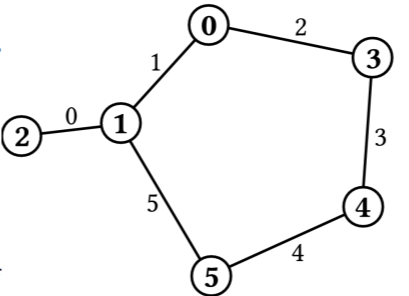
\includegraphics{garden1.png}

Есть всего два допустимых маршрута, проходящих по трём тропинкам: 
\begin{itemize}
\item $1 \rightarrow 2 \rightarrow 1 \rightarrow 0$ 
\item $5 \rightarrow 4 \rightarrow 3 \rightarrow 0$
\end{itemize}

Первый маршрут начинается возле фонтана с номером $1$. Самая красивая тропинка отсюда ведет к фонтану с номером $2$. У фонтана с номером $2$ у группы нет выбора, они должны вернуться, используя ту же тропинку. Теперь, снова находясь у фонтана с номером $1$, группа не может использовать тропинку с номером $0$, и вместо этого выбирает тропинку с номером $1$. Эта тропинка приводит их к фонтану с номером $P=0$.

Таким образом, нужно вызвать процедуру \t{answer(2)}.

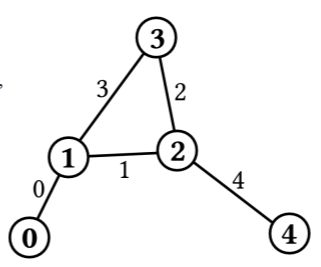
\includegraphics{garden2.png}

Для первой группы есть только один маршрут, который приводит к фонтану с номером 2, проходя по трём тропинкам: $1 \rightarrow 0 \rightarrow 1 \rightarrow 2$. Для второй группы есть два маршрута, которые приводят к фонтану с номером $2$, проходя по одной тропинке: $3 \rightarrow 2$, и $4 \rightarrow 2$. Таким образом, правильная реализация процедуры \t{count\_routes} должна сначала вызывать \t{answer(1)} чтобы сообщить ответ для первой группы, после чего вызвать \t{answer(2)}, чтобы сообщить ответ для второй группы.
